\documentclass[12pt,a4paper]{article}

%-----------------------------------
% Packages
%-----------------------------------
\usepackage[utf8]{inputenc}
\usepackage[english]{babel}
\usepackage{graphicx}
\usepackage{float}
\usepackage{geometry}
\usepackage{booktabs}
\usepackage{longtable}
\usepackage{hyperref}
\usepackage{enumitem}
\usepackage{array}

\geometry{
left=2.5cm,
right=2.5cm,
top=2.5cm,
bottom=2.5cm
}

\hypersetup{
    colorlinks=true,
    linkcolor=blue,
    citecolor=blue,
    urlcolor=blue
}

\title{
Lab 1A\\
Business Requirements Analysis\\
Retail Analytics Platform
}

\author{
Deyton Riascos Ortiz\\
Samuel Izquierdo Bonilla\\
Daniel David Garcia Restrepo\\
Mauricio Taborda Gongora
}

\date{July 31, 2026}

\begin{document}

\maketitle

\tableofcontents

\newpage

%%%%%%%%%%%%%%%%%%%%%%%%%%%%%%%%%%%%%%
\section{Introduction}

This report documents the business requirements analysis for a retail sales analytics platform (\textit{Retail Analytics}). The objective of Lab 1A is to understand the business problem, define commercial objectives, identify functional and non-functional requirements, and design a dashboard wireframe that will serve as the foundation for the ETL process to be implemented in Lab 1B \cite{dama2017}.

The project team consists of three members with defined roles following agile methodologies: a Project Manager, a Product Owner, and a Development Team member \cite{pmi2021}.

%%%%%%%%%%%%%%%%%%%%%%%%%%%%%%%%%%%%%%
\section{Business Problem Analysis}

\subsection{Problem}

The company has sales, inventory, and product data, but the information is scattered across spreadsheets and different systems. This makes it difficult for managers to get a quick and reliable view of store performance and make timely decisions.

\subsection{Importance}

Resolving this problem is important because it:
\begin{itemize}[nosep]
    \item Reduces time spent searching for information.
    \item Enables data-driven decision-making.
    \item Quickly identifies underperforming products.
    \item Facilitates tracking of goal compliance.
    \item Improves marketing campaign planning.
\end{itemize}

\subsection{Stakeholders}

\begin{table}[H]
\centering
\begin{tabular}{p{4cm} p{9cm}}
\toprule
\textbf{Stakeholder} & \textbf{Expected Benefit}\\
\midrule
Regional Managers & Monitor the performance of their stores\\
Store Managers & Analyze sales and local trends\\
Marketing Team & Adjust campaigns based on each store's performance\\
Senior Management & Obtain strategic indicators for decision-making\\
\bottomrule
\end{tabular}
\caption{Main stakeholders and their expected benefits.}
\end{table}

\subsection{Business Decisions}

With an adequate analytics platform, managers will be able to:
\begin{itemize}[nosep]
    \item Identify stores with low performance.
    \item Detect product categories with declining sales.
    \item Design promotions for specific products.
    \item Compare performance across regions.
    \item Evaluate compliance with commercial goals.
    \item Plan inventory based on sales trends.
\end{itemize}

\subsection{Missing Information}

Before designing the solution, it is necessary to ask the client:

\begin{table}[H]
\centering
\begin{tabular}{p{6cm} p{7cm}}
\toprule
\textbf{Question} & \textbf{Justification}\\
\midrule
Which indicators are priorities for management? & Define the main KPIs\\
How often do sales goals change? & Properly interpret goal compliance\\
What access levels will each user have? & Define permissions and security\\
How many stores and regions exist? & Estimate data volume\\
What system stores promotions? & Properly integrate sources\\
What format should downloadable reports have? & Meet business needs\\
What exactly does a ``successful store'' mean? & Establish evaluation criteria\\
What historical data should be retained? & Define the analysis period\\
\bottomrule
\end{tabular}
\caption{Additional questions for the client.}
\end{table}

%%%%%%%%%%%%%%%%%%%%%%%%%%%%%%%%%%%%%%
\section{Business Objectives}

\begin{table}[H]
\centering
\small
\begin{tabular}{p{5.5cm} p{8cm}}
\toprule
\textbf{Business Objective} & \textbf{Why is it Important?}\\
\midrule
Centralize sales information into a single analytical view & Reduces time spent searching for information across different files and systems\\
Monitor sales performance by region and store & Allows quickly identifying branches with best and worst performance\\
Analyze category and product performance & Helps detect low-demand products and define promotions\\
Evaluate compliance with commercial goals & Helps measure objective achievement and adjust campaigns\\
Analyze sales trends over time & Allows comparing daily, weekly, monthly, or annual performance\\
Facilitate clear and easy access to information for managers & Increases platform adoption and reduces the learning curve\\
Analyze the impact of promotions on sales & Helps measure whether campaigns are actually driving sales\\
Facilitate operational tracking of transactions & Provides day-to-day indicators such as average order value\\
\bottomrule
\end{tabular}
\caption{Business objectives and their importance.}
\end{table}

%%%%%%%%%%%%%%%%%%%%%%%%%%%%%%%%%%%%%%
\section{Analytical Questions}

\begin{table}[H]
\centering
\small
\begin{tabular}{p{7cm} p{6.5cm}}
\toprule
\textbf{Business Question} & \textbf{Information Required}\\
\midrule
What is the total sales by day, week, month, and year? & Sales transactions with date and amount\\
Which product categories generate the highest and lowest revenue? & Sales grouped by product category\\
Which products have the best and worst performance? & Quantity sold and revenue by product\\
Which stores have the best and worst performance? & Total sales by store\\
How do sales vary across regions? & Sales grouped by region\\
How have sales evolved compared to the previous month or year? & Sales history by period\\
Which stores meet or fail to meet their commercial goals? & Actual sales and goals for each store\\
What impact do promotions have on sales? & Promotion information related to sales\\
What sales trends exist by period? & Sales time series (daily, weekly, monthly)\\
What reports do managers and marketing need to download? & Consolidated sales, goals, and promotions data\\
\bottomrule
\end{tabular}
\caption{Analytical questions and the information required to answer them.}
\end{table}

%%%%%%%%%%%%%%%%%%%%%%%%%%%%%%%%%%%%%%
\section{Requirements Identification}

\subsection{Functional Requirements}

\begin{table}[H]
\centering
\small
\begin{tabular}{p{1.2cm} p{5.5cm} p{6cm}}
\toprule
\textbf{ID} & \textbf{Functional Requirement} & \textbf{Justification}\\
\midrule
FR-01 & Display total sales by day, week, month, and year & Enables commercial performance monitoring\\
FR-02 & Visualize sales by region and by store & Facilitates comparing performance across branches\\
FR-03 & Display category and product performance & Identifies high and low performing products\\
FR-04 & Allow filtering information by region, store, and time period & Facilitates specific analysis according to user needs\\
FR-05 & Display historical sales trends & Allows comparing behavior across different periods\\
FR-06 & Display goal compliance by store & Helps commercial and marketing areas evaluate results\\
FR-07 & Integrate promotion information with sales & Allows analyzing the impact of promotional campaigns\\
FR-08 & Allow report downloads & Facilitates sharing information outside the platform\\
\bottomrule
\end{tabular}
\caption{Functional requirements of the system.}
\end{table}

\subsection{Non-Functional Requirements}

\begin{table}[H]
\centering
\small
\begin{tabular}{p{1.2cm} p{5.5cm} p{6cm}}
\toprule
\textbf{ID} & \textbf{Non-Functional Requirement} & \textbf{Justification}\\
\midrule
NFR-01 & The dashboard must update information daily & The client indicated daily updates are sufficient\\
NFR-02 & The platform must be easy to use and intuitive & Some managers do not have technical knowledge\\
NFR-03 & Only authorized users will be able to access the information & Protects the company's commercial data\\
NFR-04 & Indicator loading time must not exceed 5 seconds & Improves user experience\\
NFR-05 & The platform must be available during business hours & Ensures access when managers need it\\
NFR-06 & It must be compatible with mobile devices & Some managers work while traveling\\
NFR-07 & It must allow growth in number of stores and data volume & Facilitates business scalability\\
NFR-08 & The information presented must be consistent and reliable & Prevents decisions based on incorrect data\\
\bottomrule
\end{tabular}
\caption{Non-functional requirements of the system.}
\end{table}

\begin{figure}[H]
\centering
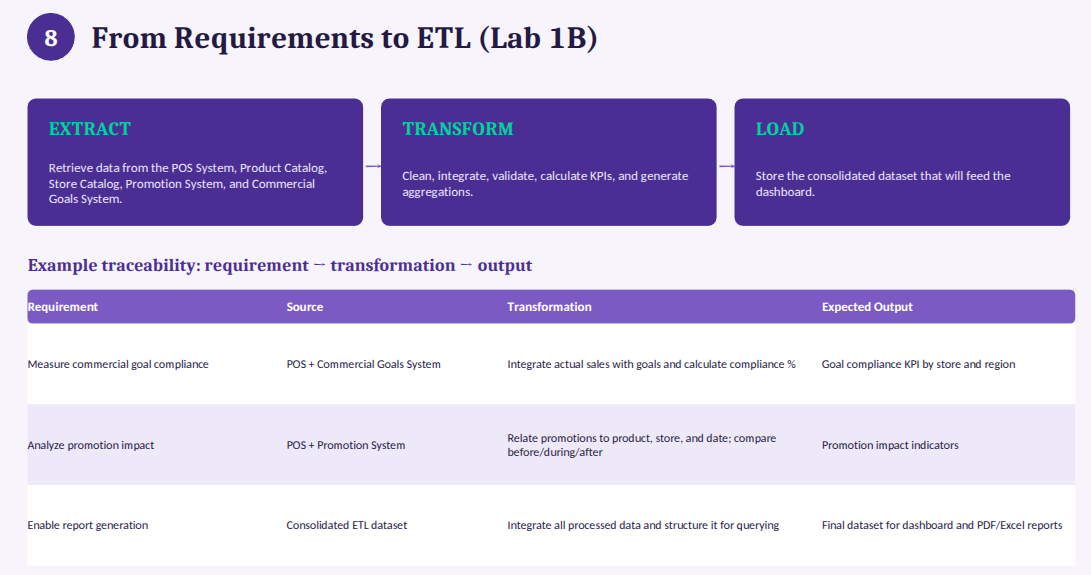
\includegraphics[width=\textwidth]{../figures/requeriments.png}
\caption{Summary of functional and non-functional requirements.}
\end{figure}

\subsection{Data Requirements}

\begin{table}[H]
\centering
\small
\begin{tabular}{p{3cm} p{3.5cm} p{3cm} p{3.5cm}}
\toprule
\textbf{Information Needed} & \textbf{Data Required} & \textbf{Possible Source} & \textbf{Why is it Needed?}\\
\midrule
Monthly Sales & Sales transactions & POS System & Calculate total sales and trends\\
Sales by Store & Store ID, date, and amount & POS System & Compare performance across branches\\
Sales by Region & Store and region information & POS + Store Catalog & Analyze geographic differences\\
Product Performance & Product catalog and sales & Catalog + POS & Identify successful products\\
Category Performance & Categories and sales & Product Catalog & Evaluate categories by revenue\\
Goal Compliance & Commercial goals and actual sales & Goals System & Measure objective achievement\\
Active Promotions & Campaigns, dates, and products & Promotion System & Analyze promotion impact on sales\\
Historical Trends & Sales history & POS System & Compare periods and detect patterns\\
\bottomrule
\end{tabular}
\caption{Data requirements for the analytics platform.}
\end{table}

\begin{figure}[H]
\centering
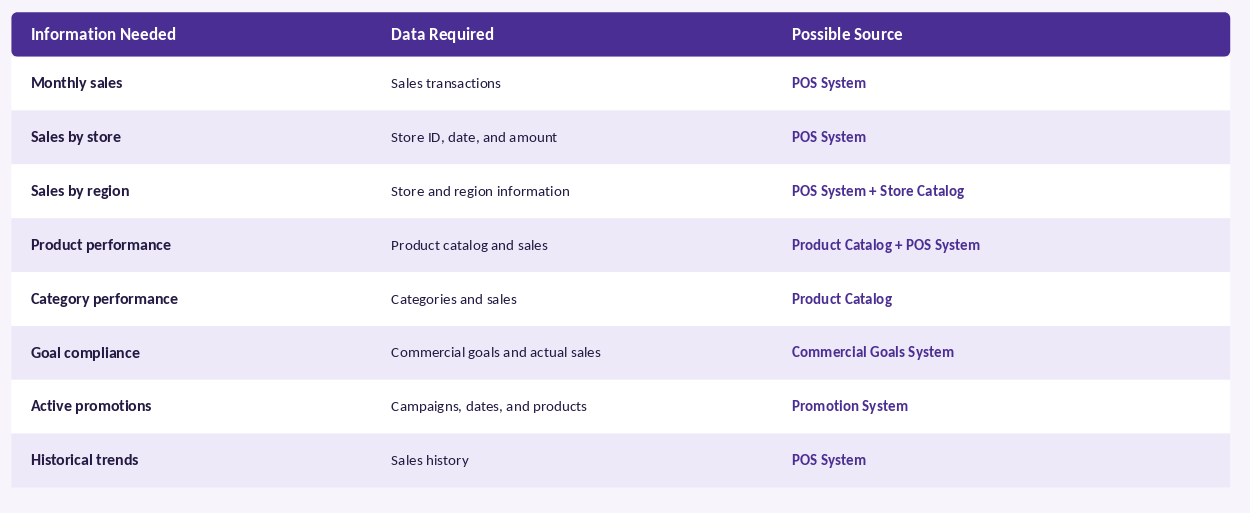
\includegraphics[width=\textwidth]{../tables/dataRequirements.png}
\caption{Data requirements table with sources and transformations.}
\end{figure}

%%%%%%%%%%%%%%%%%%%%%%%%%%%%%%%%%%%%%%
\section{User Stories}

\subsection{Story 1}

\textbf{As a} regional manager, \textbf{I want to} visualize sales of all stores in my region, \textbf{so that} I can quickly identify which ones have the best and worst performance.

\subsection{Story 2}

\textbf{As a} store manager, \textbf{I want to} view sales by product category, \textbf{so that} I can detect which products need promotions or commercial strategies.

\subsection{Story 3}

\textbf{As a} marketing team member, \textbf{I want to} visualize which stores meet their commercial goals, \textbf{so that} I can adjust advertising campaigns and strengthen underperforming stores.

\subsection{Story 4}

\textbf{As a} regional manager, \textbf{I want to} compare current sales with those from the previous month and year, \textbf{so that} I can evaluate growth or decline in commercial performance.

\subsection{Story 5}

\textbf{As a} commercial director, \textbf{I want to} download consolidated reports of sales and goal compliance, \textbf{so that} I can present them in follow-up meetings and support strategic decision-making.

\subsection{Story 6 (Added Value)}

\textbf{As a} store manager, \textbf{I want to} visualize the impact of promotions on sales, \textbf{so that} I can identify which campaigns generate the best results.

\begin{table}[H]
\centering
\small
\begin{tabular}{p{3.5cm} p{5cm} p{5cm}}
\toprule
\textbf{User} & \textbf{Decision to Make} & \textbf{Information Needed}\\
\midrule
Regional Manager & Identify stores with best and worst performance & Sales by region and by store\\
Store Manager & Decide which products need promotion & Sales by product and category\\
Marketing Team & Adjust commercial campaigns & Goal compliance and sales results\\
Commercial Director & Evaluate overall company performance & KPIs, trends, and historical comparisons\\
Regional Manager & Detect changes in sales behavior & Daily, weekly, and monthly trends\\
Store Manager & Evaluate promotion effectiveness & Promotion data and associated sales\\
\bottomrule
\end{tabular}
\caption{Decision and information needs by user role.}
\end{table}

%%%%%%%%%%%%%%%%%%%%%%%%%%%%%%%%%%%%%%
\section{KPIs}

\begin{table}[H]
\centering
\small
\begin{tabular}{p{4.5cm} p{3.5cm} p{5.5cm}}
\toprule
\textbf{Business Objective} & \textbf{KPI} & \textbf{Justification}\\
\midrule
Centralize sales information & Total Revenue & Measures the total value of sales made\\
Monitor store performance & Sales by Store & Allows comparing performance across branches\\
Analyze performance by region & Sales by Region & Facilitates geographic analysis\\
Evaluate categories and products & Sales by Category & Identifies categories with highest contribution\\
Evaluate categories and products & Top 10 Best-Selling Products & Knows the most in-demand products\\
Analyze sales trends & Sales Growth (\%) & Compares sales with previous periods\\
Evaluate goal compliance & Goal Compliance Percentage & Measures the degree of objective achievement\\
Analyze promotion impact & Sales Increase by Promotion & Evaluates impact of promotional campaigns\\
Operational tracking & Average Order Value & Average value of each purchase made\\
\bottomrule
\end{tabular}
\caption{KPIs aligned with business objectives.}
\end{table}

\subsection{KPIs requiring data from multiple systems}

The following KPIs require integrating information from more than one source:

\begin{table}[H]
\centering
\begin{tabular}{p{4cm} p{9cm}}
\toprule
\textbf{KPI} & \textbf{Systems Involved}\\
\midrule
Goal Compliance Percentage & POS System + Commercial Goals System\\
Sales Increase by Promotion & POS System + Promotion System\\
\bottomrule
\end{tabular}
\caption{KPIs requiring integration of multiple data sources.}
\end{table}

\subsection{Most difficult KPI to calculate}

The \textbf{Sales Increase by Promotion} would be the most complex KPI because:
\begin{itemize}[nosep]
    \item It requires integrating sales and promotion data from different systems.
    \item Each promotion must be related to the corresponding products, stores, and dates.
    \item To measure the impact, sales before, during, and after each campaign must be compared, avoiding attributing changes to external factors such as seasonality.
\end{itemize}

%%%%%%%%%%%%%%%%%%%%%%%%%%%%%%%%%%%%%%
\section{Dashboard Wireframe}

The lab asks to design a low-fidelity wireframe of the dashboard. The proposal includes:

\begin{figure}[H]
\centering
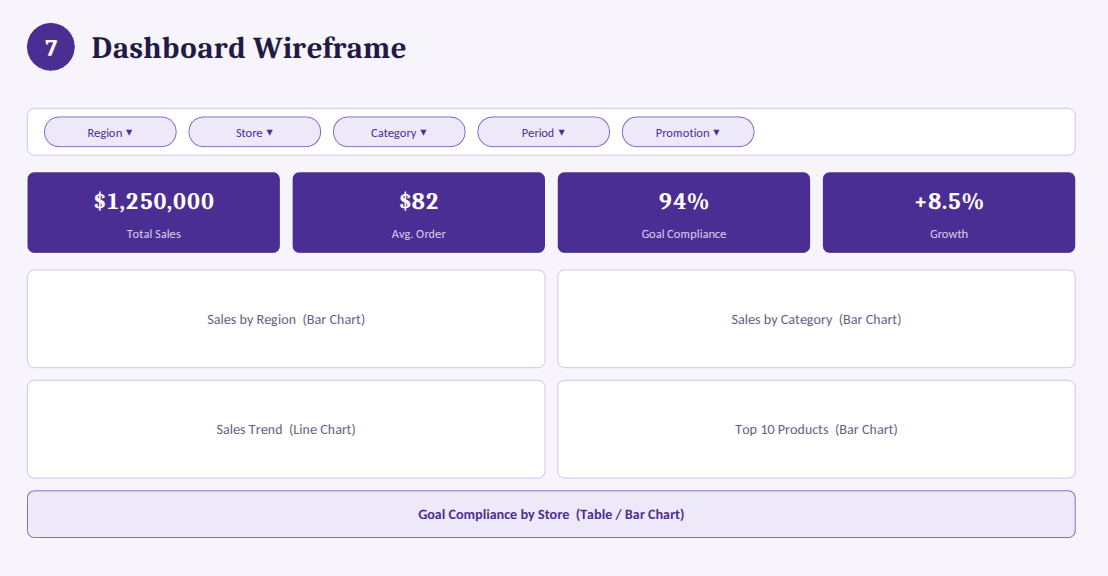
\includegraphics[width=\textwidth]{../figures/dashboardWireFame.png}
\caption{Proposed sales analytics dashboard wireframe.}
\end{figure}

\subsection{Design Justification}

\textbf{Filters:} Located at the top because they affect all displayed information. They include region, store, category, period, and promotion, responding to the client's requirements to analyze information from different perspectives.

\textbf{KPIs:} The first row presents the most important indicators: total sales, average order value, goal compliance, and growth percentage. These are metrics that managers need to check immediately.

\textbf{Charts:} Four main visualizations:
\begin{itemize}[nosep]
    \item Bars by Region: Compare performance across regions.
    \item Bars by Category: Identify categories with best and worst performance.
    \item Trend Line: Analyze sales evolution over time.
    \item Top 10 Products: Identify products with the highest sales volume.
\end{itemize}

\textbf{Goal Compliance:} A separate chart or table because the client indicated that the marketing area needs to evaluate which stores meet their commercial objectives.

\textbf{Export:} A section for exporting reports in PDF or Excel, since the client mentioned the need to download reports.

The dashboard follows a logical reading flow: filters (define the context) $\rightarrow$ KPIs (overview) $\rightarrow$ charts (deep analysis) $\rightarrow$ details (goal compliance) $\rightarrow$ export (share information) \cite{kimball2013}.

%%%%%%%%%%%%%%%%%%%%%%%%%%%%%%%%%%%%%%
\section{Preparing for Lab 1B}

\begin{table}[H]
\centering
\small
\begin{tabular}{p{3.2cm} p{2.8cm} p{3.8cm} p{3.2cm}}
\toprule
\textbf{Business Requirement} & \textbf{Data Source} & \textbf{Transformation Needed} & \textbf{Expected Output}\\
\midrule
Visualize total sales by period & POS System & Clean records, convert dates, calculate totals & Dataset with sales aggregated by period\\
Analyze sales by region & POS + Store Catalog & Join tables by store ID, group by region & Sales consolidated by region\\
Compare store performance & POS + Store Catalog & Relate sales with store information & Metrics per branch\\
Analyze product/category performance & POS + Product Catalog & Relate products with categories & Indicators by category and product\\
Measure goal compliance & POS + Goals System & Integrate actual sales with assigned goals & Goal compliance KPI by store\\
Analyze promotion impact & POS + Promotion System & Relate promotions with sales before/during/after & Impact indicators\\
Analyze historical trends & POS (historical) & Sort chronologically, generate aggregations & Time series for charts\\
Enable report generation & Consolidated ETL dataset & Integrate all processed data & Final dataset for dashboard and reports\\
\bottomrule
\end{tabular}
\caption{Business requirements mapped to the ETL process for Lab 1B.}
\end{table}

\subsection{Transformation Justification}

The proposed transformations correspond to the classic stages of an ETL process \cite{inmon2005}:

\begin{table}[H]
\centering
\begin{tabular}{p{4cm} p{9cm}}
\toprule
\textbf{Transformation} & \textbf{Objective}\\
\midrule
Data Cleaning & Remove incomplete, duplicate, or inconsistent records\\
Format Conversion & Standardize dates, currencies, and data types\\
Source Integration & Combine information from POS, catalogs, goals, and promotions\\
Aggregation & Calculate summary metrics by period, region, or store\\
KPI Calculation & Generate metrics ready for dashboard consumption\\
\bottomrule
\end{tabular}
\caption{ETL transformations and their objectives.}
\end{table}

\subsection{Relationship with the ETL Process}

\begin{table}[H]
\centering
\begin{tabular}{p{2.5cm} p{10.5cm}}
\toprule
\textbf{ETL} & \textbf{Application in This Case}\\
\midrule
\textbf{Extract} & Retrieve data from POS System, Product Catalog, Store Catalog, Promotion System, and Commercial Goals System\\
\textbf{Transform} & Clean, integrate, validate, calculate KPIs, and generate aggregations\\
\textbf{Load} & Store the consolidated dataset that will feed the analysis dashboard\\
\bottomrule
\end{tabular}
\caption{Application of ETL stages to the case study.}
\end{table}

%%%%%%%%%%%%%%%%%%%%%%%%%%%%%%%%%%%%%%
\section{Reflection}

\subsection{Why is a Dashboard not the first step?}

No. This activity showed that building a dashboard is actually one of the last visible steps, not the first one. Before any table, chart, or wireframe can be designed, the team had to understand the business problem, identify stakeholders, translate their needs into objectives and analytical questions, and only then define functional, non-functional, and data requirements.

This prior work made clear that the data sources involved (POS System, Product Catalog, Store Catalog, Commercial Goals System, and Promotion System) need to be integrated before any KPI can be trusted. If the team had started by designing the dashboard, it likely would have missed requirements such as mobile access, security levels, or the need to relate promotions to sales.

In short, the dashboard is the visible outcome of the process, but the real first step is understanding the business problem and the data needed to solve it \cite{dama2017}.

%%%%%%%%%%%%%%%%%%%%%%%%%%%%%%%%%%%%%%
\section{AI Prompts}

As part of this activity, the team used an AI assistant as a support tool to organize ideas, check for completeness, and refine the wording of the deliverables. All content was reviewed, validated, and adjusted by the team before being included in this report.

\begin{table}[H]
\centering
\small
\begin{tabular}{p{2cm} p{4cm} p{7cm}}
\toprule
\textbf{Activity} & \textbf{Prompt Purpose} & \textbf{Example Prompt}\\
\midrule
General & Translate and clarify instructions & ``Translate this lab statement into clear, simple terms and list what each activity is asking for''\\
Activity 1 & Identify gaps in requirements & ``Based on this client transcript, what information is missing that a data engineer should ask about?''\\
Activity 2 & Turn needs into objectives & ``Help me phrase these client needs as business objectives, separate from any technical solution''\\
Activity 3 & Convert objectives into questions & ``For each business objective, suggest a business question and the information required to answer it''\\
Activity 4 & Distinguish requirement types & ``Given these business objectives, suggest functional, non-functional, and data requirements, and explain the difference''\\
Activity 5 & Draft user stories & ``Write user stories in the As a/I want/So that format for a regional manager, store manager, and marketing member''\\
Activity 6 & Define and justify KPIs & ``Suggest KPIs aligned with these business objectives, and identify which ones require combining data from more than one system''\\
Activity 7 & Structure the wireframe & ``Suggest a logical layout for a sales dashboard wireframe, including filters, KPIs, charts, and an export section''\\
Review & Check consistency & ``Review whether these business objectives, KPIs, and requirements are consistent with each other''\\
\bottomrule
\end{tabular}
\caption{AI prompts used during the lab development.}
\end{table}

%%%%%%%%%%%%%%%%%%%%%%%%%%%%%%%%%%%%%%
\section{Conclusions}

Lab 1A allowed a complete analysis of business requirements for the retail sales analytics platform. The business problem, stakeholders, commercial objectives, analytical questions, functional and non-functional requirements, user stories, KPIs, and a dashboard wireframe were clearly identified.

It is concluded that the integration of multiple data sources (POS System, Product Catalog, Store Catalog, Commercial Goals System, and Promotion System) is a fundamental requirement for the platform to answer all the business questions raised. The ETL process to be implemented in Lab 1B will be the mechanism to achieve this integration.

%%%%%%%%%%%%%%%%%%%%%%%%%%%%%%%%%%%%%%
\section{References}

\bibliographystyle{plain}
\bibliography{../referencias}

\end{document}
